Figure~\ref{fig:cross-temp} shows cross-temperature transfer results for the 6-generator LOGO pipeline.
We evaluate four train$\rightarrow$test temperature conditions using Qwen3-1.7B data regenerated at $t{=}1.0$ (remaining five generators retain $t{=}0.7$).\footnote{The $t{=}1.0$ data uses top-$p{=}0.95$ (vs.\ $p{=}0.9$ for other configurations); this difference may contribute to the observed degradation beyond the temperature effect alone.}

\begin{figure}[t]
\centering
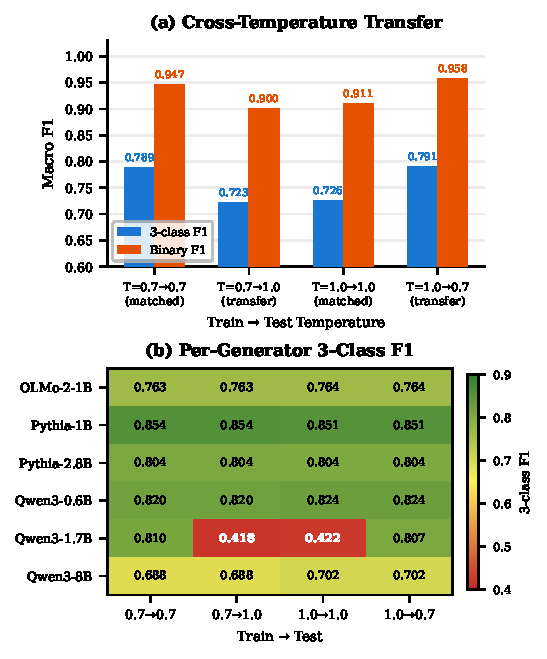
\includegraphics[width=\columnwidth]{fig_appendix_cross_temp.pdf}
\caption{Cross-temperature transfer evaluation (6-gen LOGO). (a) Overall F1 by train$\rightarrow$test temperature condition. Matched conditions (0.7$\rightarrow$0.7, 1.0$\rightarrow$1.0) outperform cross-temperature transfer, with 0.7$\rightarrow$1.0 showing the largest degradation ($-6.6$\,pp in 3-class F1). (b) Per-generator 3-class F1 heatmap: Qwen3-1.7B shows dramatic degradation under cross-temperature conditions (0.418) while other generators remain stable. The temperature mismatch disproportionately affects the generator whose data was regenerated.}
\label{fig:cross-temp}
\end{figure}

Key observations from the cross-temperature analysis:

\begin{enumerate}[nosep]
\item \textbf{Matched-temperature robustness}: Both $t{=}0.7$ and $t{=}1.0$ matched conditions yield comparable performance (3-class F1: 0.789 vs.\ 0.726), with the gap attributable to weaker depth signal at high temperature rather than classifier degradation.

\item \textbf{Asymmetric transfer}: Training at $t{=}1.0$ and testing at $t{=}0.7$ (F1\,=\,0.791) transfers well, but the reverse (0.7$\rightarrow$1.0, F1\,=\,0.723) degrades. This asymmetry reflects the information structure: features learned from high-variance (high-temperature) data generalize to low-variance settings, but not vice versa.

\item \textbf{Generator-specific vulnerability}: Qwen3-1.7B, the only generator with temperature-mismatched test data, drops to F1\,=\,0.418 under cross-temperature conditions while all other generators maintain F1 $>$ 0.76. This confirms that depth features are calibrated to the specific decoding regime.

\item \textbf{Binary transfer for the mismatched generator}: For Qwen3-1.7B (the only generator with actual temperature mismatch), binary F1 drops from 0.948 to 0.713 under 0.7$\rightarrow$1.0 transfer but recovers in the reverse direction (1.0$\rightarrow$0.7: 0.948), consistent with the asymmetric pattern in Item 2. The aggregate binary range (0.900--0.958) is inflated by five generators whose data is identical across conditions.
\end{enumerate}
